\section{The LHCb detector}

Before introducing the \lhcb detector, it is helpful to first define a cartesian coordinate system.
The $z$ direction is defined by the \lhc beam pipe, where the $pp$ interaction point is located
at $z=0$, and the \lhcb detector extends in the positive $z$ direction.
Often, the terms \emph{upstream} and \emph{downstream} are useful to refer to being in the
negative or positive $z$ direction, respectively.
An vector originating at the interaction point has an angle $\theta$ with respect to the $z$ axis.
The $x$ coordinate defines the horizontal direction, and $y$ is vertical.

The \lhcb detector is a single arm forward spectrometer, reminiscent of a fixed target experiment,
with an acceptance of $1.8<\eta<4.9$, where pseudorapidity defined as
\begin{equation}
  \eta = -\log\left[\tan\left(\frac\theta2\right)\right].
\end{equation}
This configuration was chosen because in hadronic interactions \bbbar pairs are predominantly
produced with momentum vectors aligned close to the beam line.
Figure~\ref{fig:lhcb:bbbar} shows the $\theta$ distribution of the \bquark and \bquarkbar quarks
produced in a $pp$ interaction at $8\tev$.

\begin{figure}
  \begin{center}
    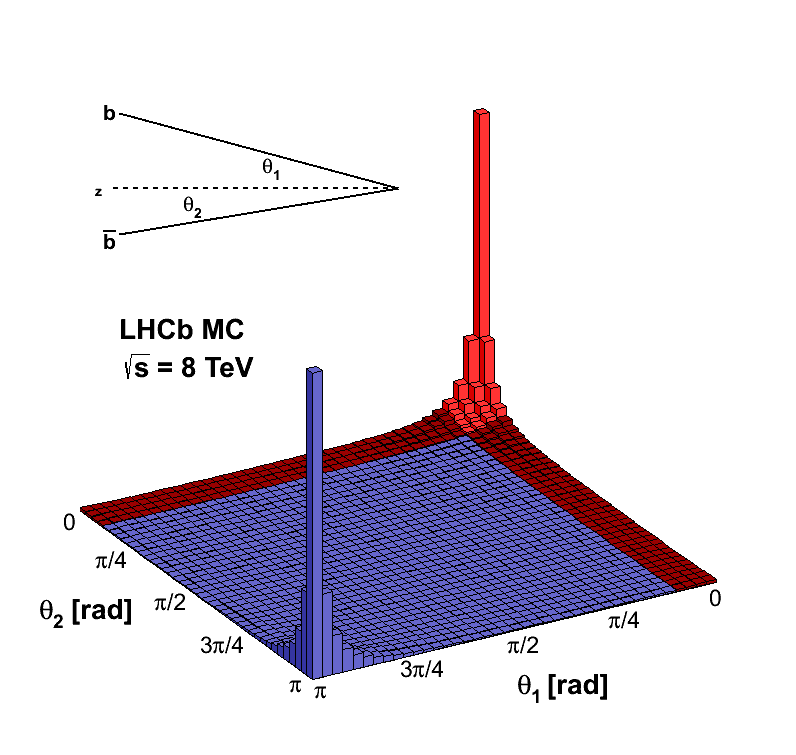
\includegraphics[width=0.5\textwidth]{acceptance}
  \end{center}
  \caption[Simulated production of $b\bquarkbar$ pairs and the LHCb acceptance]
  {\small
    Simulation of the production of \bquark and \protect\bquarkbar quarks leaving the $pp$
    interaction point with angles $\theta_1$ and $\theta_2$, respectively.
    It is clear that the majority of of these particles have momentum vectors that are close to the
    beam pipe, which justifies the geometry of the \lhcb detector.
    The dark red indicates the \lhcb acceptance region.
  }
  \label{fig:lhcb:bbbar}
\end{figure}



%this angle; the acceptance of \lhcb covers approximately $25\,\%$ of \bbbar pairs, this is also indicated.
%Using the coordinate system where $z$ is defined by the \lhc beam pipe,
%%($z=0$ being the interaction point),
%\lhcb has an acceptance in pseudorapidity, $\eta$, of $1.8<\eta<4.9$.  %(\lesssim)
%Pseudorapidity is defined as $-\log\left(\tan\tfrac\theta2\right)$, where $\theta$ is the angle
%between the $z$ axis and the momentum vector of some particle emerging from the interaction point.
%The interaction point is at $z=0$ and the positive $z$ direction is referred to as downstream.
%The $x$ and $y$ axes are then defined by the horizontal and vertical directions respectively.
%Figure~\ref{fig:lhcb:lhcb} is a schematic diagram of the \lhcb indicating the coordinate system and
%subdetectors.
%A schematic diagram of the \lhcb detector is shown in Fig~\ref{fig:lhcb:lhcb}.



%Spatial coordinates of charged particles traversing the detector are recorded as hits in the
%tracking systems.
%Particle momentum is deduced by their curvature in the $x$ direction when then pass through the
%detector region which is immersed in a magnet field.
%This field has an integrated strength of $4\,\mathrm{Tm}$ and is provided by a large conventional
%magnet.
%Other subdetector systems include two Cherenkov detectors used for particle identification;
%calorimeters, which are used for triggering; and muon stations which are used for identifying and
%triggering muons.

The analyses included in this thesis deal exclusively with charged particle final states.
A charged particle leaving the interaction region is measured with the tracking system, which
consists of a vertex detector and four planar tracking stations.
Part of the detector volume is immersed in a magnet field, provided by a large conventional magnet
with an integrated field strength of $4\,\mathrm{Tm}$.
This bends particles in the $x$ direction, providing information about charge and, in conjunction
with the tracking system, momentum.
Two Cherenkov detectors are used for offline particle identification, allowing \lhcb to distinguish
between, for example, pions and kaons.
Further downstream of the tracking systems is the calorimetry system, which is primarily used for
triggering; but is also used for some particle identification.
The final subdetector system that a particle might traverse is the muon system.
This consists of five stations --- which are only be penetrated by the most energetic muons --- and
is used for tracking, triggering, and \pid.
Figure~\ref{fig:lhcb:lhcb} is a schematic diagram of the \lhcb detector, indicating the coordinate
system and subdetector modules.
The following sections provide further information about the \lhcb detector.


\begin{figure}
  \begin{center}
    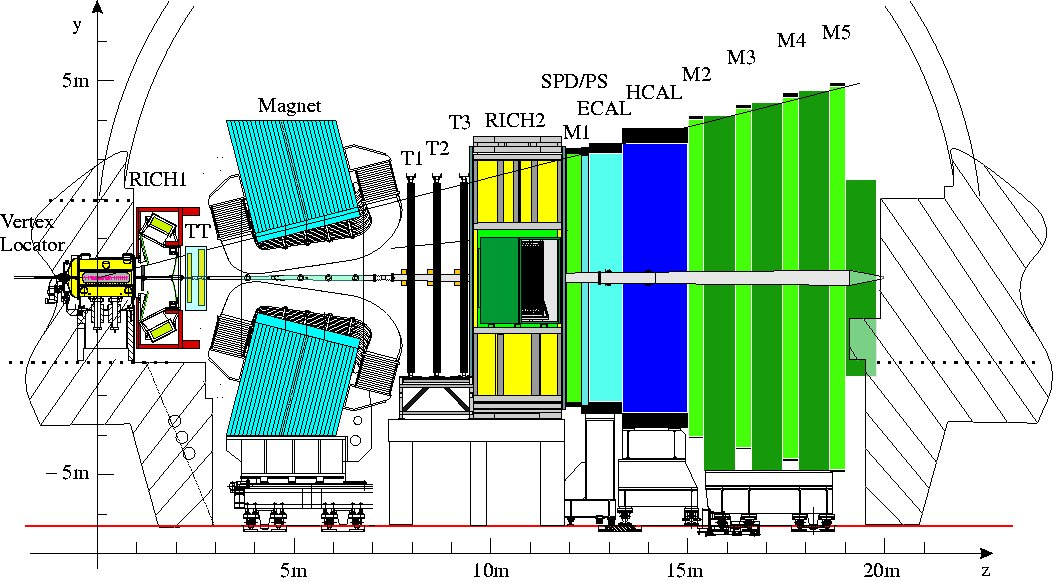
\includegraphics[width=\textwidth]{LHCb_detector}
  \end{center}
  \caption[Diagram of the LHCb detector]
  {\small
    Schematic diagram of the \lhcb detector with labeled subdetectors and coordinate system, the
    $x$ direction comes out of the page.
  }
  \label{fig:lhcb:lhcb}
\end{figure}


